\ifdefined\handout
  \documentclass[handout]{beamer}
\else
  \documentclass{beamer}
\fi

\usetheme{boxes}
\usecolortheme{structure}

\setbeamertemplate{footline}[frame number]

\ifdefined\handout
\definecolor{beamer@structure@color}{rgb}{0,0,0}
\setbeamertemplate{navigation symbols}{}
\setbeamercolor{normal text}{fg=black,bg=white}
\setbeamertemplate{frametitle}{\vskip 15pt\color{black}
\def\myhrulefill{\leavevmode\leaders\hrule height 1pt\hfill\kern 0pt}
\headingfont\insertframetitle\par\vskip-8pt\myhrulefill}
\else
\definecolor{beamer@structure@color}{rgb}{1,1,1}
\setbeamertemplate{navigation symbols}{}
\setbeamercolor{normal text}{fg=white,bg=black}
\setbeamertemplate{frametitle}{\vskip 15pt\color{white}
\def\myhrulefill{\leavevmode\leaders\hrule height 1pt\hfill\kern 0pt}
\headingfont\insertframetitle\par\vskip-8pt\myhrulefill}
\fi

\usepackage{amsmath,amssymb}

\newcommand{\NN}{\mathbb{N}}
\newcommand{\ZZ}{\mathbb{Z}}

\DeclareMathOperator{\mcd}{mcd}
\DeclareMathOperator{\mcm}{mcm}

\usepackage[spanish]{babel}

\usepackage{tikz-cd}
\usetikzlibrary{babel}
\usetikzlibrary{calc}

\usepackage{framed}

\newcommand{\dfn}{\mathrel{\mathop:}=}
\newcommand{\rdfn}{=\mathrel{\mathop:}}

\usepackage{mathspec}
\setsansfont[BoldFont={IBM Plex Sans Bold}, ItalicFont={IBM Plex Sans Italic}]{IBM Plex Sans}
\setmonofont[BoldFont={IBM Plex Mono Bold}, ItalicFont={IBM Plex Mono Italic}]{IBM Plex Mono}
\setmathrm[BoldFont={IBM Plex Sans Bold}, ItalicFont={IBM Plex Sans Italic}]{IBM Plex Sans}
\newfontfamily\headingfont[]{IBM Plex Sans Bold}

\setbeamercovered{transparent=10}


\begin{document}

\begin{frame}[plain,noframenumbering]
  \textbf{INTRODUCCIÓN A LA TEORÍA DE NÚMEROS}

  Alexey Beshenov $\mid$ \texttt{cadadr.org}

  \vfill

  \begin{center}\huge\headingfont
    ALGORITMO DE EUCLIDES EXTENDIDO,

    \vspace{0.5em}

    IDENTIDAD DE BÉZOUT,

    \vspace{0.5em}

    ECUACIÓN DIOFÁNTICA

    AX + BY = C
  \end{center}

  \vfill
\end{frame}

\begin{frame}[plain,noframenumbering]

  \vfill

  \begin{center}\huge\headingfont
    MOTIVACIÓN:

    \vspace{0.5em}

    ECUACIÓN DIOFÁNTICA

    AX + BY = C
  \end{center}

  \vfill
\end{frame}

\begin{frame}
  \frametitle{ECUACIONES DIOFÁNTICAS}

  \onslide<2->{Ecuaciones algebraicas (en dos o más variables) de las que se
    buscan soluciones enteras.}

    \begin{itemize}
    \item<3-> $x^2 + y^2 = z^2$ --- \textbf{ternas pitagóricas}.

      \onslide<4->{$(x,y,z) = (3,4,5), \, (5,12,13), \, (7,24,25), \, \ldots$}

    \item<5-> $x^4 + y^4 = z^2$\onslide<6->{ --- no hay soluciones enteras (Fermat).}

    \item<7-> $y^2 = x^3 - 2$ --- una \textbf{curva elíptica}.
      \onslide<8->{$(x,y) = (3, \pm 5)$.}

    \item<9-> $x^2 - 3 y^2 = 1$ --- \textbf{ecuación de Pell}.

      \onslide<10->{$(x,y) = (1, 0), \, (2, 1), \, (7, 4), \, (26, 15), \, (97, 56), \, \ldots$}

    \item<11-> $x^n + y^n = z^n$ --- \textbf{ecuación de Fermat}.

      \onslide<12->{No hay soluciones con $x,y,z \ne 0$ para $n \ge 3$ (Wiles, 1994).}

    \item<13-> $x^a - y^b = 1$ para $a,b > 1$, $x,y > 0$.

      \onslide<14->{\textbf{Conjetura de Catalan}: la única posibilidad es
        $3^2 - 2^3 = 1$ (Mihăilescu, 2002).}
    \end{itemize}
\end{frame}

\begin{frame}
  \begin{center}
    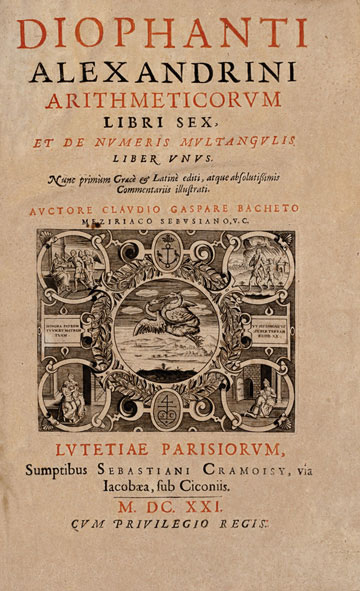
\includegraphics[width=.4\textwidth]{diofanto-aritmetica.jpg}

    «Aritmética» (edición latín de 1621) \\
    Diofanto de Alejandría (siglo III d.C.)
  \end{center}
\end{frame}

\begin{frame}
  \frametitle{LA ECUACIÓN DIOFÁNTICA MÁS SENCILLA}

  \onslide<2->{Para $a,b,c \in \ZZ$ fijos

  {\huge \[ ax + by = c \]}}
\end{frame}

\begin{frame}
  \frametitle{EJEMPLO: $5x + 3y = 1$}

  \begin{center}
    \begin{tikzpicture}[x=0.3cm,y=0.3cm, font=\footnotesize]
      \foreach \i in {-10,...,10} \draw[\ifdefined\handout black!50\else black!50\fi] (-10,\i) -- (+10,\i);
      \foreach \i in {-10,...,10} \draw[\ifdefined\handout black!50\else black!50\fi] (\i,-10) -- (\i,+10);

      \draw[->,\ifdefined\handout black\else white\fi] (-11,0) -- (11,0) node[right] {$x$};
      \draw[->,\ifdefined\handout black\else white\fi] (0,-11) -- (0,11) node[above] {$y$};

      \draw (6.8, -11) -- (-6.4, +11);

      \draw (-4,7) node[circle,fill,inner sep=1.25pt] {};
      \draw (-1,2) node[circle,fill,inner sep=1.25pt] {};
      \draw (2,-3) node[circle,fill,inner sep=1.25pt] {};
      \draw (5,-8) node[circle,fill,inner sep=1.25pt] {};
    \end{tikzpicture}
  \end{center}
\end{frame}

\begin{frame}
  \frametitle{EJEMPLO: $6x + 3y = 1$}

  \begin{center}
    \begin{tikzpicture}[x=0.3cm,y=0.3cm, font=\footnotesize]
      \foreach \i in {-10,...,10} \draw[\ifdefined\handout black!50\else black!50\fi] (-10,\i) -- (+10,\i);
      \foreach \i in {-10,...,10} \draw[\ifdefined\handout black!50\else black!50\fi] (\i,-10) -- (\i,+10);

      \draw[->,\ifdefined\handout black\else white\fi] (-11,0) -- (11,0) node[right] {$x$};
      \draw[->,\ifdefined\handout black\else white\fi] (0,-11) -- (0,11) node[above] {$y$};

      \draw (17/3, -11) -- (-16/3, +11);
    \end{tikzpicture}
  \end{center}
\end{frame}

\begin{frame}
  \frametitle{UN ACERTIJO}

  \onslide<2->{Encuentre una solución entera de

  {\huge \[ 28x + 30y + 31z = 365 \]}}
\end{frame}

\begin{frame}[plain,noframenumbering]

  \vfill

  \begin{center}\huge\headingfont
    EL ALGORITMO DE EUCLIDES EXTENDIDO

    \vspace{1em}

    Y LA IDENTIDAD DE BÉZOUT
  \end{center}

  \vfill
\end{frame}

\begin{frame}
  \frametitle{ALGORITMO DE EUCLIDES CLÁSICO}

  \begin{itemize}
  \item<2-> Pongamos $r_0 \dfn a$, $r_1 \dfn b$.

  \item<3-> Calculamos las divisiones con residuo
    $$r_{i-1} = q_n\,r_n + r_{i+1}$$
    hasta obtener $r_{i+1} = 0$.

  \item<4->
    $\mcd (a,b) = \mcd (r_0,r_1) = \mcd (r_1,r_2) = \mcd (r_2,r_3) = \cdots =
    \mcd (r_i,r_{i+1}) = \mcd (r_i,0) = r_i$.
  \end{itemize}
\end{frame}

\begin{frame}
  \frametitle{ALGORITMO DE EUCLIDES EXTENDIDO}

  \begin{align*}
    \onslide<2->{r_0} & \onslide<2->{\dfn a,} & \onslide<2->{s_0} & \onslide<2->{\dfn 1,} & \onslide<2->{t_0} & \onslide<2->{\dfn 0,} \\
    \onslide<3->{r_1} & \onslide<3->{\dfn b,} & \onslide<3->{s_1} & \onslide<3->{\dfn 0,} & \onslide<3->{t_1} & \onslide<3->{\dfn 1.}
  \end{align*}

  \onslide<4->{Calculamos}
  \begin{align*}
    \onslide<5->{r_{i+1}} & \onslide<5->{= r_{i-1} - q_i\,r_i,} \\
    \onslide<6->{s_{i+1}} & \onslide<6->{= s_{i-1} - q_i\,s_i,} \\
    \onslide<7->{t_{i+1}} & \onslide<7->{= t_{i-1} - q_i\,t_i.}
  \end{align*}

  \onslide<8->{\begin{framed}
    $$r_i = a s_i + b t_i.$$
  \end{framed}}
\end{frame}

\begin{frame}
  \frametitle{ALGORITMO DE EUCLIDES EXTENDIDO}

  \begin{align*}
    \onslide<2->{r_0} & \onslide<2->{= a \underbrace{s_0}_{= 1} + b \underbrace{t_0}_{= 0} = a,} \\
    \onslide<3->{r_1} & \onslide<3->{= a \underbrace{s_1}_{= 0} + b \underbrace{t_1}_{= 1} = b,} \\
    \\
    \onslide<4->{r_{i+1}} & \onslide<4->{= r_{i-1} - q_i\,r_i} \\
                      & \onslide<5->{\stackrel{\text{H.I.}}{=} (a\,s_{i-1} + b\,t_{i-1}) - q_i\,(a\,s_i + b\,t_i)} \\
                      & \onslide<6->{= a\,(s_{i-1} - q_i\,s_i) + b\,(t_{i-1} - q_i\,t_i)} \\
                      & \onslide<7->{\stackrel{\text{def.}}{=} a s_{i+1} + b t_{i+1}. \qed}
  \end{align*}

\end{frame}

\begin{frame}
  \frametitle{COROLARIO: IDENTIDAD DE BÉZOUT}

  \onslide<2->{Para cualesquiera $a,b \in \ZZ$ existen $x,y \in \ZZ$ tales que
    \[ \tag{*} ax + by = \mcd (a,b). \]}

  \onslide<3->{Para $(a,b) \ne (0,0)$ el mcd es el mínimo número positivo de la forma
    $ax + by$:
    $$\mcd (a,b) = \min \{ ax + by > 0 \mid x,y \in \ZZ \}.$$}

  \onslide<4->{\textbf{Demostración}.}

  \onslide<5->{(*) --- por el algoritmo de Euclides extendido.}

  \onslide<6->{Para $d \dfn \mcd (a,b)$ tenemos $d \mid a$, $d \mid b$.
    $$d \mid (ax + by), \quad 0 < ax + by < d$$}
  \onslide<7->{---¡imposible! \qed}
\end{frame}

\begin{frame}
  \frametitle{EJEMPLO: $\mcd (21,13)$}

  \begin{align*}
    \onslide<2->{r_0} & \onslide<2->{= 21,} & \onslide<2->{s_0} & \onslide<2->{= 1,} & \onslide<2->{t_0} & \onslide<2->{= 0,} \\
    \onslide<3->{r_1} & \onslide<3->{= 13,} & \onslide<3->{s_1} & \onslide<3->{= 0,} & \onslide<3->{t_1} & \onslide<3->{= 1,} \\
    \onslide<4->{r_2} & \onslide<4->{= 8,} & \onslide<4->{s_2} & \onslide<4->{= s_0 - q_1\,s_1 = 1,} & \onslide<4->{t_2} & \onslide<4->{= t_0 - q_1\,t_1 = -1,} & \onslide<4->{(q_1 = 1)} \\
    \onslide<5->{r_3} & \onslide<5->{= 5,} & \onslide<5->{s_3} & \onslide<5->{= s_1 - q_2\,s_2 = -1,} & \onslide<5->{t_3} & \onslide<5->{= t_1 - q_2\,t_2 = 2,} & \onslide<5->{(q_2 = 1)} \\
    \onslide<6->{r_4} & \onslide<6->{= 3,} & \onslide<6->{s_4} & \onslide<6->{= s_2 - q_3\,s_3 = 2,} & \onslide<6->{t_4} & \onslide<6->{= t_2 - q_3\,t_3 = -3,} & \onslide<6->{(q_3 = 1)} \\
    \onslide<7->{r_5} & \onslide<7->{= 2,} & \onslide<7->{s_5} & \onslide<7->{= s_3 - q_4\,s_4 = -3,} & \onslide<7->{t_5} & \onslide<7->{= t_3 - q_4\,t_4 = 5,} & \onslide<7->{(q_4 = 1)} \\
    \onslide<8->{r_6} & \onslide<8->{= 1,} & \onslide<8->{s_6} & \onslide<8->{= s_4 - q_5\,s_5 = 5,} & \onslide<8->{t_6} & \onslide<8->{= t_4 - q_5\,t_5 = -8,} & \onslide<8->{(q_5 = 1)} \\
    \onslide<9->{r_7} & \onslide<9->{= 0.}
  \end{align*}

  \onslide<10->{Conclusión:
    $$21\cdot 5 + 13\cdot(-8) = 1.$$}
\end{frame}

% \begin{frame}
%   \frametitle{ELECCIÓN DE COEFICIENTES DE BÉZOUT}

%   \begin{itemize}
%   \item Número infinito de $x$ e $y$ tales que $ax + by = \mcd (a,b)$.
%     \[ 21\cdot 5 + 13\cdot (-8) = 21\cdot (-8) + 13\cdot 13 = 21\cdot 18 + 13\cdot (-29) = \cdots \]

%   \item Supongamos que $a,b > 0$ y $\mcd (a,b) \ne \min \{ a, b \}$.

%     En el algoritmo de Euclides extendido se cumple
%     \[
%       |s_i| \le \left\lfloor \frac{b}{2 \mcd (a,b)} \right\rfloor,
%       \quad
%       |t_i| \le \left\lfloor \frac{a}{2 \mcd (a,b)} \right\rfloor.
%     \]

%   \item $a x + b y = \mcd (a,b)$ posee única solución $(x_0,y_0)$ con
%     \[
%       |x_0| \le \left\lfloor \frac{b}{2 \mcd (a,b)} \right\rfloor,
%       \quad
%       |y_0| \le \left\lfloor \frac{a}{2 \mcd (a,b)} \right\rfloor.
%     \]
%   \end{itemize}
% \end{frame}

% \begin{frame}
%   \frametitle{EJEMPLO}

%   \[ a = 21, ~ b = 13, ~ x = 5, ~ y = -8. \]

%   \[ 21\cdot 5 + 13\cdot (-8) = 1. \]

%   \begin{align*}
%     \left\lfloor \frac{b}{2 \mcd (a,b)} \right\rfloor & =
%     \left\lfloor \frac{13}{2} \right\rfloor = 6, \\
%     \left\lfloor \frac{a}{2 \mcd (a,b)} \right\rfloor & =
%     \left\lfloor \frac{21}{2} \right\rfloor = 10.
%   \end{align*}
% \end{frame}

\begin{frame}[plain,noframenumbering]
  \vfill

  \begin{center}\huge\headingfont
    VOLVIENDO A LAS ECUACIONES DIOFÁNTICAS LINEALES
  \end{center}

  \vfill
\end{frame}

\begin{frame}
  \frametitle{TEOREMA}

  \onslide<2->{Pongamos $d = \mcd (a,b)$.}

  \begin{itemize}
  \item<3-> $ax + by = c$ tiene solución si y solo si $d \mid c$.

    \onslide<4->{\textbf{Condición necesaria}.

      Si $ax + by = c$, entonces $d\mid a$ y $d\mid b$ implica $d \mid c$.}

    \onslide<5->{\textbf{Condición suficiente}.

      $ax + by = d$ tiene solución por la identidad de Bézout.

      Si $c = dc'$, entonces $a\,(xc') + b\,(yc') = c$.}

  \item<6-> Si $(x_0,y_0)$ es una solución, entonces todas las demás son
    \[
      x = x_0 + \frac{b}{d}\,t,
      \quad
      y = y_0 - \frac{a}{d}\,t,
      \quad
      t \in \ZZ.
    \]
  \end{itemize}
\end{frame}

\begin{frame}
  \frametitle{SOLUCIONES EN GENERAL}
  \onslide<2->{\begin{framed}
      \[
        x = x_0 + \frac{b}{d}\,t,
        \quad
        y = y_0 - \frac{a}{d}\,t.
      \]
    \end{framed}}

  \onslide<3->{\[
      a\cdot \left(x_0 + \frac{b}{d}\,t\right) +
      b\cdot \left(y_0 - \frac{a}{d}\,t\right) =
      ax_0 + by_0 = c.
    \]}
\end{frame}

\begin{frame}
  \frametitle{SOLUCIONES EN GENERAL (CONT.)}
  \begin{gather*}
    \onslide<2->{ax + by = ax_0 + by_0 = c,} \\
    \onslide<3->{\frac{a}{d}\,x + \frac{b}{d}\,y = \frac{a}{d}\,x_0 + \frac{b}{d}\,y_0} \onslide<4->{\iff \frac{a}{d}\,(x - x_0) = \frac{b}{d}\,(y_0 - y).}
  \end{gather*}

  \begin{multline*}
    \onslide<5->{\frac{a}{d} \mid
      \mcd \left(\frac{a}{d}\,(y_0-y), \frac{a}{d}\,(x-x_0)\right)} \\
    \onslide<6->{= \mcd \left(\frac{a}{d}\,(y_0-y), \frac{b}{d}\,(y_0 - y)\right)} \\
    \onslide<7->{= (y_0 - y)\cdot \mcd \underbrace{\left(\frac{a}{d}, \frac{b}{d}\right)}_{= 1}} \onslide<8->{= (y_0 - y).}
  \end{multline*}

  \[
    \onslide<9->{\frac{a}{d} \mid (y_0 - y),} \quad
    \onslide<10->{\frac{b}{d} \mid (x-x_0) \quad \text{ (similar)}.}
  \]
\end{frame}

\begin{frame}
  \frametitle{SOLUCIONES EN GENERAL (CONT.)}

  \begin{align*}
    \onslide<2->{\frac{b}{d} \mid (x-x_0)} & \onslide<2->{\iff x = x_0 + \frac{b}{d}\,t,} \\
    \onslide<3->{\frac{a}{d} \mid (y_0 - y)} & \onslide<3->{\iff y = y_0 - \frac{a}{d}\,t'.}
  \end{align*}

  \begin{multline*}
    \onslide<4->{ax_0 + by_0 = ax + by} \\
    \onslide<5->{= a\,\left(x_0 + \frac{b}{d}\,t\right) + b\,\left(y_0 - \frac{a}{d}\,t'\right)} \\
    \onslide<6->{= ax_0 + by_0 + \frac{ab}{d}\,(t - t').}
  \end{multline*}

  \onslide<7->{Conclusión: $t = t'$.}
\end{frame}

\begin{frame}
  \frametitle{EJEMPLO}

  \onslide<2->{\[ 5x + 3y = 1. \]}

  \onslide<3->{Algoritmo de Euclides extendido (o adivinando):
    \[ (x_0,y_0) = (-1,2). \]}

  \onslide<4->{Todas las soluciones:
    \[
      (x,y) = \left(x_0 + \frac{b}{d}\,t, y_0 - \frac{a}{d}\,t\right)
      = (-1 + 3t, \, 2 - 5t), \quad t \in \ZZ.
    \]}

  \onslide<5->{\[
    \ldots, \,
    (-7, 12), \,
    (-4, 7), \,
    (-1, 2), \,
    (2, -3), \,
    (5, -8), \,
    \ldots
  \]}
\end{frame}

\begin{frame}[plain,noframenumbering]
  \vfill

  \begin{center}\huge\headingfont
    VOLVIENDO AL ACERTIJO
  \end{center}

  \vfill
\end{frame}

\begin{frame}
  \frametitle{EL ACERTIJO}

  \begin{itemize}
  \item<2-> Buscamos una solución entera de
    $28x + 30y + 31z = 365$.

  \item<3-> Identidad de Bézout:
    $$28\cdot (-1) + 30\cdot 1 = 2.$$

  \item<4-> Otra identidad de Bézout:
    $$2\cdot (-15) + 31\cdot 1 = 1.$$

  \item<5-> Combinando:
    $$28\cdot 15 + 30\cdot (-15) + 31\cdot 1 = 1.$$

  \item<6-> Respuesta:
    $$28\cdot 5475 + 30\cdot (-5475) + 31\cdot 365 = 365.$$
  \end{itemize}
\end{frame}

\begin{frame}
  \frametitle{LA VERDADERA RESPUESTA}

  \onslide<2->{$$28x + 30y + 31z = 365$$}

  \onslide<3->{\begin{center}
    \renewcommand{\arraystretch}{1.25}
    \begin{tabular}{ccc}
      \hline
      \textbf{enero} & \textbf{febrero} & \textbf{marzo} \\
      31 días & 28 días & 31 días \\
      \hline
      \textbf{abril} & \textbf{mayo} & \textbf{junio} \\
      30 días & 31 días & 30 días \\
      \hline
      \textbf{julio} & \textbf{agosto} & \textbf{septiembre} \\
      31 días & 31 días & 30 días \\
      \hline
      \textbf{octubre} & \textbf{noviembre} & \textbf{diciembre} \\
      31 días & 30 días & 31 días \\
      \hline
    \end{tabular}
  \end{center}}

  \onslide<4->{$$(x,y,z) = (1, 4, 7).$$}
\end{frame}


\begin{frame}
  \frametitle{EJERCICIOS}

  \begin{itemize}
  \item<2-> Demuestre que $\mcd (a, a+b) \mid b$.

  \item<3-> Calcule $\mcd (a+1, a-1)$ para $a \in \ZZ$.

  \item<4-> Calcule $\mcd (a+b, a-b)$ para $a,b \in \ZZ$ \\
    en términos de $\mcd(a,b)$.

  \item<5-> Calcule $\mcd (9a+4, 2a+1)$ para $a \in \ZZ$.

  \item<6-> ¿Cuándo $a_1 x_1 + \cdots + a_n x_n = c$ tiene una solución?

  \item<7-> Demuestre que $\mcd (a_1,\ldots,a_n)$ es el mínimo número positivo
    de la forma $a_1 x_1 + \cdots + a_n x_n$ con $x_1, \ldots, x_n \in \ZZ$.
  \end{itemize}
\end{frame}

\begin{frame}[plain,noframenumbering]

  \vfill

  \begin{center}\huge\headingfont
    ¡GRACIAS POR SU ATENCIÓN!
  \end{center}

  \vfill
\end{frame}
\end{document}
